\subsection{Antena dla promieniowania THz o~działaniu opartym na wzbudzeniu modu falowodowego}
\label{subart:antenaThz}
Projektowana antena promieniowania THz powinna nie tylko zapewniać selektywność reakcji na promieniowanie E-M z~wąskiego zakresu długości fali, co można uzyskać przy użyciu mechanizmów opisanych w~podrozdziale \ref{subart:rezo-grating}. Jej podstawowym zadaniem jest umożliwiać wzbudzenie detektora zlokalizowanego w~małym obszarze za pomocą promieniowania padającego na dowolną część anteny. Zastosowanie siatki dyfrakcyjnej jest najwydajniejszą metodą na sprzężenie fali E-M z~zakresu THz do podkładu z~półprzewodnika. Możliwa jest wydajność sprzężenia sięgająca nawet 80\%\cite{roux2002grating}.  Schemat układu anteny, wraz z~podkładem w~którym umieszczony jest detektor promieniowania THz w~postaci tranzystora polowego, przedstawia rysunek \ref{fig:schem-podklad-falo}.
\begin{figure}[tb]
	\centering
	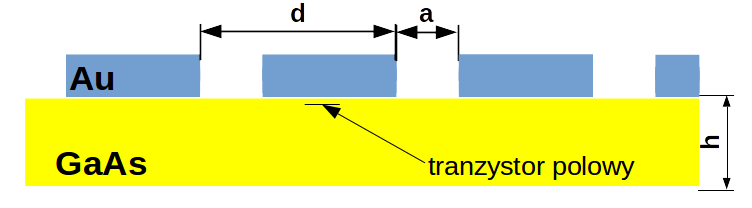
\includegraphics[width=\textwidth]{images/thz/schemat-podklad-falo.png}
	\caption{Schemat detektora promieniowania THz na tranzystorze polowym umieszczonym w~falowodzie z~$GaAs$ z~naniesioną złotą siatką dyfrakcyjną}
	\label{fig:schem-podklad-falo}
\end{figure}

Rozkład pola na rysunku \ref{fig:consrcl525} nie zapewnia transportu promieniowania E-M w~kierunku tranzystora polowego. Możliwy jest jednak transport energii z~wykorzystaniem falowodu planarnego tworzonego przez podkład z~$GaAs$. Ze względu na konieczność stosowania polaryzacji TM w~stukturach opisywanych w~części \ref{subart:rezo-grating} w~tej części skupiamy się również jedynie na tego typu oświetleniu. Przyjmijmy obecnie, że propagacja fali wzdłuż falowodu odbywa się w~kierunku $z$. Wtedy trzy składowe pola E-M opisujące propagującą falę to $E_x$,$E_z$ i~$H_y$, które zgodnie z~równaniami Maxwella spełniają układ równań różniczkowych:
\begin{equation}
\begin{gathered}
	\frac{\partial E_x}{\partial z} - \frac{\partial E_z}{\partial x} = -i \mu \omega H_y,\\	
	\frac{\partial H_y}{\partial x} = i~\omega \varepsilon E_z, \\
	- \frac{\partial H_y}{\partial z} = i~\omega \varepsilon E_x.
\end{gathered}
\end{equation}
Z powyższych równań wyprowadzić można równanie różniczkowe drugiego rzędu, będące jedną z~postaci równania Hemlhotza, dla składowej $H_y$ w~postaci
\begin{equation}
	[ \frac{\partial^2}{\partial x^2} + \frac{\partial^2}{\partial z^2} + \omega^2 \mu_0 \varepsilon (x) ] H_y = 0,
	\label{eq:waveguide-tm}
\end{equation}
w którym $\varepsilon(x)$ jest współczynnikiem załamania ośrodków. W rozważanym przypadku
\begin{equation}
\varepsilon(x)=  
\begin{cases} 
	1, & \mbox{dla } x>h\mbox{ powyżej podkładu z~GaAs } \\ 
	\varepsilon_{\textrm{GaAs}}, & \mbox{dla } 0<x<h\mbox{ wewnątrz podkładu z~GaAs} \\
	\varepsilon_x,	&	\mbox{dla } x<0\mbox{ poniżej podkładu z~GaAs}.\\
\end{cases}
\end{equation}
W powyższym równaniu współczynnik załamania poniżej struktury został opisany jako $\varepsilon_x$, co pozwala w~dalszej analize rozważać falowody w~których $GaAs$ zostało umieszczone na innym materiale. Szukając rozwiązań równania (\ref{eq:waveguide-tm}) w~postaci fal płaskich, propagujących się wewnątrz rdzenia ($0<x<h$) wzdłuż osi z:
\begin{equation}
	H_y(x,z)=H_y(x) \textrm{exp}(-i \beta z),
\end{equation}
oraz w~postaci fal zanikających na zewnątrz rdzenia, otrzymujemy równanie zwyczajne
\begin{equation}
	\frac{d H_y^2(x)}{dx^2} + [ \omega^2 \mu \varepsilon - \beta^2 ] H_y = 0,
\end{equation}
dla którego stosując standardowe warunki zszycia otrzymujemy równanie dyspersyjne modów prowadzonych w~postaci~\cite{petykiewicz1989podstawy}:
\begin{equation}
tg( \kappa h)=\frac{\kappa [ \delta (\frac{n_{\textrm{GaAs}}}{n_x})^2 + \gamma n_{\textrm{GaAs}}^2 ]}{\kappa^2 - \gamma \delta (\frac{n_{\textrm{GaAs}}}{n_x })^2},
\label{eq:tm-disp}
\end{equation}
gdzie przez $n_{\textrm{GaAs}}$ i~$n_x$ oznaczono odpowiednio współczynnik załamania warstwy arsenku galu, oraz podkładu. Wprowadzono również dodatkowe ozanczenia w~postaci
\begin{equation}
	\begin{gathered}
		\delta=\sqrt{\beta^2-\omega^2 \mu_0 \varepsilon_0 \varepsilon_x},\\
		\gamma=\sqrt{\beta^2-\omega^2 \mu_0 \varepsilon_0},\\
		\kappa=\sqrt{\omega^2 \mu_0 \varepsilon_0 \varepsilon_{\textrm{GaAs}} - \beta^2}.
	\end{gathered}
\end{equation}

Wszystkie wartości $\beta$ spełniające  równanie (\ref{eq:tm-disp}) są dopuszczalnymi wartościami składowej wektora falowego w~kierunku propagacji. W ten sposób efektywne współczynniki załamania modów TM w~falowodzie planarnym można obliczyć jako $n_{\textrm{eff}}=\frac{\beta}{k_0}$. Rozwiązanie powyższego równania możliwe jest jedynie na drodze numerycznej~(lub graficznie). W przypadku rozważanych podkładów z~$GaAs$, $h=400$~$\mu m$, możliwe wartości efektywnego współczynnika załamania przedstawia wykres \ref{fig:gaas-effn}. Różne współczynniki $n_{\textrm{eff}}$ odpowiadające tej samej długości fali wynikają z~wielomodowego charakteru falowodu tworzonego przez podkład $GaAs$. Dopasowanie pędowe między modem prowadzonym w~falowodzie, a falą padającą wymaga dodania odpowiedniego pędu do fali padającej przez siatkę dyfrakcyjną, co dla składowych wektora falowego możemy zapisać jako
\[
k_{i \parallel} + l \frac{2\pi}{d} = k_0 \cdot n_{\textrm{eff,m}}, 
\]
gdzie przez $k_{i \parallel}$ oznaczono składową wektora falowego równoległą do kierunku propagacji w~falowodzie, $l$ jest liczbą całkowitą odpowiadającą rzędowi ugięcia na siatce dyfrakcyjnej, a $n_{\textrm{eff,m}}$ jest efektywnym współczynnikiem m-tego modu falowodowego. W przypadku padania normalnego pęd fali padającej w~kierunku propagacji w~falowodzie wynosi zero. Szczególnie interesujący jest również przypadek wzbudzenia modu za pomocą pierwszego rzędu dyfrakcyjnego siatki, ponieważ dla niego uzyskamy największą wydajność, dlatego po uproszczeniu z~powyższego równania możemy wyprowadzić
\begin{equation}
d=\frac{2 \pi}{k_0 \cdot n_{\textrm{eff,m}}}.
\label{eq:d-do-wzbudzenia}
\end{equation}
Na podstawie powyższego wzoru przygotowano wykres zależności okresu siatki $d$ potrzebnej do wzbudzenia kolejnych modów falowodowych w~zależności od długości fali dla której pracować ma antena. Wyniki tych obliczeń przedstawia wykres \ref{fig:d-lusok}.

\begin{figure}
\begin{subfigure}{0.5\textwidth}
        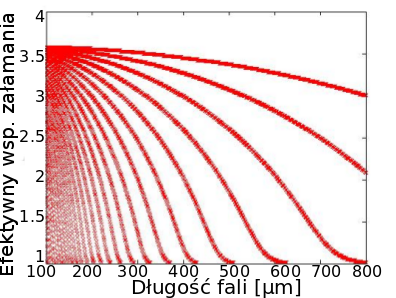
\includegraphics[width=\textwidth]{images/thz/gaas-neffeps.png}
	\caption{}
	\label{fig:gaas-effn}
\end{subfigure}
\begin{subfigure}{0.5\textwidth}
        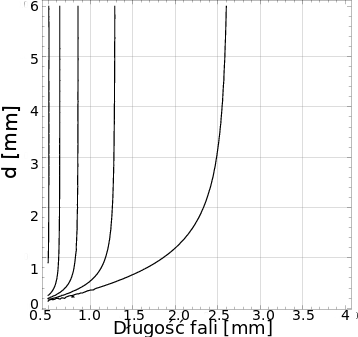
\includegraphics[width=\textwidth]{images/antenaThz/d_lambda.png}
	\caption{}
	\label{fig:d-lusok}
\end{subfigure}
\caption{Wyniki rozwiązania problemu falowodu planarnego o~grubości $h=$400~$\mu$m z~GaAs.  (a) Zależność $n_{\textrm{eff}}$ od długości fali, (b)~wykres łączący okres siatki dyfrakcyjnej z~długością fali dla której pracuje antena. }
\end{figure}



Na podstawie przeprowadzonych obliczeń zaproponowano siatkę dla źródła o~częstotliwości $f=300$~GHz ($\lambda\approx 1$~mm) o~grubości $H=1$~$\mu$m i~okresie $d=729$~$\mu$m. W strukturach wytwarzanych eksperymentalnie pod podkładem $GaAs$ znajduje się warstwa $Au$ o~grubości 1~$\mu$m, którą w~symulacji metodą FDTD traktujemy jako doskonały przewodnik. Na rysunku \ref{fig:consrc_1d_f300Ghz} przedstawiono rozkład gęstości energii wewnątrz zaproponowanej struktury. Wyniki symulacji komputerowych potwierdzają  możliwość propagacji promieniowania E-M z~zakresu subterahercowego w~kierunku detektora w~zaprojektowanym układzie. Niemal bezstratna propagacja promieniowania z~tego zakresu w~półprzewodnikach została potwierdzona w~pracach eksperymentalnych~\cite{roux2002grating}.

\begin{figure}[tb]
	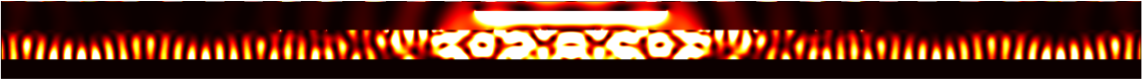
\includegraphics[width=\textwidth]{images/thz/consrc_siatka1d_300GHz_d729um.png}
	\caption{Uzyskany za pomocą symulacji metodą FDTD, uśredniony rozkład gęstości energii pola elektromagnetycznego wewnątrz falowodu z~$GaAs$, na którym umieszczono antenę w~postaci siatki dyfrakcyjnej o~$d=$729~$\mu$m oświetloną pod kątem normalnym za pomocą źródła o~częstotliwości 300~GHz.  }
	\label{fig:consrc_1d_f300Ghz}
\end{figure}

\begin{figure}[tb]
	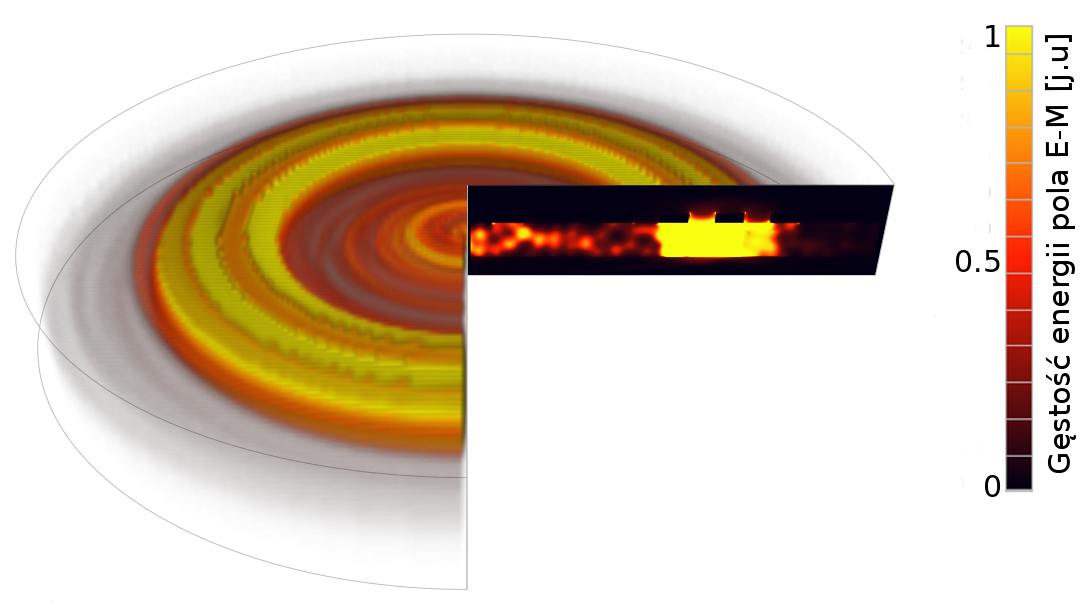
\includegraphics[width=\textwidth]{images/antenaThz/tort.png}
	\caption{Rozkład energii pola E-M uzyskany w~symulacji metodą BOR FDTD wewnątrz falowodu planarnego z~siatką o~geometrii cylindrycznej umieszczoną na podkładzie z~$GaAs$. Wynik symulacji znajduje się w~przekroju przedstawionym na rysunku. Obrazowe przejście do geometrii cylindrycznej uzyskano przez wizualizację średniej wartości w~danym punkcie falowodu.}	
	\label{fig:concent_modfalo}
\end{figure}

Bazując na pracach numerycznych dotyczących  jednowymiarowych siatek dyfrakcyjnych pozwalających na wzbudzenie modów falowodowych w~podkładach z~$GaAs$ przeanalizowane zostało działanie analogicznych falowodów opartych na cylindrycznych siatkach dyfrakcyjnych. Ze względu na wzbudzenie modów falowodowych o~kierunku propagacji prostopadłym do pasków siatki dyfrakcyjnej uzyskujemy częściową koncentrację promieniowania w~obszarze detektora. Odpowiedni eksperyment numeryczny został przeprowadzony przy użyciu metody FDTD we współrzędnych cylindrycznych, szerzej opisanej w~podrozdziale \ref{subart:borfdtd}. Wyniki symulacji przedstawione na rysunku \ref{fig:concent_modfalo} odpowiadają strukturze z~$GaAs$ o~rozmiarach 10x10mm pokrytej siatką dyfrakcyjną o~okresie $d=538$~$\mu$m i~otworach o~szerokości $250$~$\mu$m (współczynnik wypełnienia $f=0.53$), która została oświetlona promieniowaniem o~długości fali $\lambda=2.52$~mm. W ten sposób potwierdzono możliwość wykorzystania tego typu struktur do konstrukcji anten dla detektorów promieniowania THz umieszczonych wewnątrz podkładu z~$GaAs$~\cite{Stolarek2011}.

